\chapter{}
\label{lecture4}
\section{Изопериметрические задачи.}
\label{lecture4section1}
Переходим к изучению нового типа задач, в которых на допустимые функции накладывается требование типа $\int\limits_a^b G(x,y,y')\,dx=l$, где $l$ --- заданное число, а $G(x,y,y')$ --- некоторая известная функция. Рассмотрим пример.

\noindent\emph{Задача о равновесии тяжёлой не растяжимой нити.}\\
Пусть тяжёлая нить подвешена в точках $(a,y_0)$, $(b,y_1)$.

\tikzset{every picture/.style={line width=0.75pt}} %set default line width to 0.75pt        

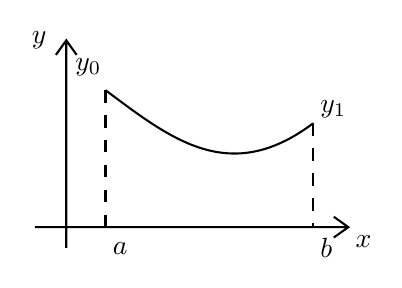
\begin{tikzpicture}[x=0.75pt,y=0.75pt,yscale=-1,xscale=1]
	%uncomment if require: \path (0,142); %set diagram left start at 0, and has height of 142
	
	%Shape: Axis 2D [id:dp3826559288358311] 
	\draw  (57,105) -- (208,105)(72.1,15) -- (72.1,115) (201,100) -- (208,105) -- (201,110) (67.1,22) -- (72.1,15) -- (77.1,22)  ;
	%Curve Lines [id:da9287316532875318] 
	\draw    (91,39) .. controls (123,63) and (151,85) .. (191,55) ;
	%Straight Lines [id:da8746375236016641] 
	\draw  [dash pattern={on 4.5pt off 4.5pt}]  (91,39) -- (91,105.5) ;
	%Straight Lines [id:da625541993436806] 
	\draw  [dash pattern={on 4.5pt off 4.5pt}]  (191,55) -- (191,105.5) ;
	
	% Text Node
	\draw (93,110.9) node [anchor=north west][inner sep=0.75pt]    {$a$};
	% Text Node
	\draw (193,108.9) node [anchor=north west][inner sep=0.75pt]    {$b$};
	% Text Node
	\draw (210,107.4) node [anchor=north west][inner sep=0.75pt]    {$x$};
	% Text Node
	\draw (54,9.4) node [anchor=north west][inner sep=0.75pt]    {$y$};
	% Text Node
	\draw (75,22.4) node [anchor=north west][inner sep=0.75pt]    {$y_{0}$};
	% Text Node
	\draw (193,42.4) node [anchor=north west][inner sep=0.75pt]    {$y_{1}$};
	
	
\end{tikzpicture}

Ясно, что её положение будет отвечать минимальному значению потенциальной энергии\footnote[1]{В этом смысле задача похожа на задачу о равновесии балки, только здесь нет изгибающего момента, но есть условие нерастяжимости.}
\begin{gather*}
	E[y]=\int\limits_a^b g\cdot\rho\cdot\sqrt{1+y^{\prime2}}\cdot y\,dx,\quad y(a)=y_0,\ y(b)=y_1,\quad\text{при условии не растяжимости}\\
	\int\limits_a^b\sqrt{1+y^{\prime2}}\,dx=l,\text{ где $l$ --- длина нити.}
\end{gather*}	
Надо найти $\min E[y]$ при описанных здесь условиях.

Сформулируем теперь общую постановку задачи
\begin{multline*}
	\text{Пусть }\J[y]=\int\limits_a^b F(x,y,y')\,dx,\ F\in\Cfn{2},\;x\in[a,b],\ |y| <M,\ y'\text{ --- любое},\\
	\K=\left\{y(x)|y\in\Cfn[{[a,b]}]{1},\ y(a)=y_0,\;y(b)=y_1,\ |y|<M,\ \int\limits_a^b G(x,y,y')\,dx=l\right\}_{\displaystyle.}
\end{multline*}
Надо найти $\min\limits_{y\in\K}\,\J[y]$.
Пусть 
\begin{equation*}
	\hfill\J_1[y]\eqdef\int\limits_a^b G(x,y,y')\,dx.\hfill
\end{equation*}
Будем предполагать, что ни одна из функций $y(x)\in\K$ не является экстремалью функционала $\J_1[y]$, то есть не удовлетворяет уравнению
\begin{equation}
	\label{l4:eq:1}
	\hfill G_y-\der{}{x}G_{y'}\equiv0.\hfill
\end{equation}
Если это не так, то есть $\exists y\in\K$, для которого~\eqref{l4:eq:1} выполняется, то тогда, считая, что функционал $\J_1[y]$ принимает на экстремалях экстремальные значения, получаем, что $\J_1[y]=l$ --- экстремальное значение. Но это равенство должно выполняться на любой функции из $\K$. Значит, весь класс \K{} в этом случае состоит из экстремалей функционала $\J_1[y]$. Но экстремаль --- в общем случае --- одна. Поэтому при выполнении~\eqref{l4:eq:1} мы получаем, что как правило, весь класс \K{} вырождается в одну функцию и задача на $\min\limits_{y\in\K}\,\J[y]$ теряет смысл.

Введём понятие допустимого изменения для рассматриваемой задачи. Оно в данном случае определяется не стандартно, что вызвано особенностями задачи. 
\begin{_def}
	Пусть $y(x)$ --- минимайзер рассматриваемой задачи. Функцию 
	\begin{equation*}
		\hfill\eta(x)\eqdef t\cdot\eta_1(x)+\alpha(t)\cdot\eta_2(x)\hfill
	\end{equation*}
	назовём \textbf{допустимым изменением}, если удаётся найти такую функцию $\alpha(t)$, $\alpha(0)=0$ и такую функцию $\eta_2(x)$, что $\tilde{y}\eqdef y+\eta(x)\in\K$, при $|t|\ll1$ и любых $\eta_1(x)$.
\end{_def}

Построим $\eta(x)$. Функции $\eta_1(x)$ и $\eta_2(x)$ берём из $\Cfn[{[a,b]}]{1}$, $\eta_i(a)=\eta_i(b)=0$, $i=1,2$. Попробуем обеспечить выполнение условия $\J[\tilde{y}]=l$. Положим
\begin{equation*}
	\hfill\Psi(t,\alpha)\eqdef\int\limits_a^b \overbrace{G\big(x,\underbrace{y+t\cdot\eta_1+\alpha(t)\cdot\eta_2}_{\tilde{y}},\underbrace{y'+t\cdot\eta'_1+\alpha(t)\cdot\eta'_2}_{\tilde{y}'}\big)}^{\widetilde{G}}\,dx.\hfill
\end{equation*}
Нам надо найти $\eta_2$ и функцию $\alpha(t)$ так, чтобы при $\forall\eta_1$ и $|t|\ll1$
\begin{equation}
	\label{l4:eq:2}
	\hfill\Psi(t,\alpha(t))\equiv l,\quad|t|\ll1.\hfill
\end{equation}
Попробуем из~\eqref{l4:eq:2} найти $\alpha(t)$ в окрестности $t=0$, $\alpha=0$, зная, что, очевидно, при $t=0$, ${\alpha(0)=0}$~\eqref{l4:eq:2} выполняется. По теореме о неявных функциях для этого надо, чтобы $\Psi_{\alpha}(0,0)\neq0$. Имеем
\begin{multline}
	\label{l4:eq:3}
	\left.\pder{\Psi(t,\alpha)}{\alpha}\right|_{\substack{t=0\\\alpha=0}}=\left.\int\limits_a^b\left(\widetilde{G}_{\tilde{y}}\cdot\eta_2+\widetilde{G}_{\tilde{y}'}\cdot\eta'_2\right)\,dx\right|_{\substack{t=0\\\alpha=0}}=\int\limits_a^b\left({G}_{{y}}\cdot\eta_2+{G}_{y'}\cdot\eta'_2\right)\,dx=\\
	=\int\limits_a^b\left(G_y-\der{}{x}G_{y'}\right)\cdot\eta_2\,dx+G_{y'}\cdot\eta_2\mathop{\Big|}\limits_a^b=\int\limits_a^b\left(G_y-\der{}{x}G_{y'}\right)\cdot\eta_2\,dx.
\end{multline}
Если бы правая часть~\eqref{l4:eq:3} равнялась нулю при $\forall\eta_2$, $\eta_2\in\Cfn[{[a,b]}]{1}$, $\eta_2(a)=\eta_2(b)=0$, то в силу леммы Лагранжа выполнялось бы~\eqref{l4:eq:1}. Но~\eqref{l4:eq:1} --- не верно по предположению. Значит мы можем найти $\eta_2$ так, что
\begin{equation}
	\label{l4:eq:4}
	\hfill\left.\pder{\Psi(t,\alpha)}{\alpha}\right|_{\substack{t=0\\\alpha=0}}\neq0.\hfill
\end{equation}
Выберем такую функцию $\eta_2(x)$ и зафиксируем её. После этого в силу~\eqref{l4:eq:4} по теореме о неявных функциях из равенства~\eqref{l4:eq:2}, \emph{верного при  $t=0$, $\alpha=0$}, мы находим $\alpha(t)$, $|t|\ll1$, обеспечивая тем самым выполнение изопериметрического условия. Таким образом, при выбранных $\alpha=\alpha(t)$ и $\eta_2$ функция $\eta=t\cdot\eta_1(x)+\alpha(t)\cdot\eta_2(x)$ --- допустимое изменение.

Для дальнейшего нам понадобится $\displaystyle\left.\pder{\Psi(t,\alpha)}{t}\right|_{\substack{t=0\\\alpha=0}}$. Чтобы найти эту величину достаточно в~\eqref{l4:eq:3} заменить $\eta_2$ на $\eta_1$ и мы получим 
\begin{equation}
	\label{l4:eq:5}
	\hfill\left.\pder{\Psi(t,\alpha)}{t}\right|_{\substack{t=0\\\alpha=0}}=\int\limits_a^b\left(G_y-\der{}{x}G_{y'}\right)\cdot\eta_1\,dx.\hfill
\end{equation}

Возвратимся теперь к нашему доказательству. Так как $\tilde{y}=y+\eta\in\K$, то поскольку $y$ --- минимайзер, то 
\begin{equation}
	\label{l4:eq:6}
	\hfill\J[y+\eta]\geqslant\J[y].\hfill
\end{equation} 
Если положить $\phi(t)\eqdef\J[y+t\cdot\eta_1+\alpha(t)\cdot\eta_2]$, то $\phi(0)=\J[y]$ и~\eqref{l4:eq:6} означает, что 
\begin{equation}
	\label{l4:eq:7}
	\hfill\phi(t)\geqslant\phi(0).\hfill
\end{equation} 
Значит, функция $\phi(t)$ принимает минимальное значение при $t=0$, и поэтому 
\begin{equation}
	\label{l4:eq:8}
	\hfill\left.\der{\phi}{t}\right|_{t=0}=0.\hfill
\end{equation} 
Вычислим
\begin{multline}
	\label{l4:eq:9}
	\left.\der{\phi}{t}\right|_{t=0}=\left.\der{\J[y+t\cdot\eta_1+\alpha(t)\cdot\eta_2]}{t}\right|_{t=0}=\left.\der{}{t}\int\limits_a^b \overbrace{F\big(x,\underbrace{y+t\cdot\eta_1+\alpha(t)\cdot\eta_2}_{\tilde{y}},\underbrace{y'+t\cdot\eta'_1+\alpha(t)\cdot\eta'_2}_{\tilde{y}'}\big)}^{\widetilde{F}}\,dx\right|_{t=0}=\\
	=\left.\int\limits_a^b\left[\widetilde{F}_{\tilde{y}}\cdot\big(\eta_1+\alpha'(t)\cdot\eta_2\big)+\widetilde{F}_{\tilde{y}'}\cdot\big(\eta'_1+\alpha'(t)\cdot\eta'_2\big)\right]\,dx\right|_{t=0}=\\
	=\int\limits_a^b\left[{F}_{{y}}\cdot\big(\eta_1+\alpha'(0)\cdot\eta_2\big)+{F}_{y'}\cdot\big(\eta'_1+\alpha'(0)\cdot\eta'_2\big)\right]\,dx=0.
\end{multline}
Обычное интегрирование по частям показывает, что
\begin{equation}
	\label{l4:eq:10}
	\hfill\int\limits_a^b F_{y'}\cdot\big(\eta'_1+\alpha'(0)\cdot\eta'_2\big)\,dx=-\int\limits_a^b\der{}{x}F_{y'}\cdot\big(\eta_1+\alpha'(0)\cdot\eta_2\big)\,dx.\hfill
\end{equation}
Далее находим $\alpha'(0)$. Так как 
\begin{equation*}
	\hfill\Psi(t,\alpha(t))\equiv l,\quad|t|\ll1,\hfill
\end{equation*}
то дифференцируя это тождество по $t$ получим
\begin{equation*}
	\hfill\left.\der{\Psi}{t}\right|_{t=0}=\Psi_t+\Psi_{\alpha}\cdot\alpha'(0)=0.\hfill
\end{equation*}
Откуда
\begin{equation}
	\label{l4:eq:11}
	\hfill\alpha'(0)=-\frac{\Psi_t(0,0)}{\Psi_{\alpha}(0,0)}=-\frac{\displaystyle\int\limits_a^b\left(G_y-\der{}{x}G_{y'}\right)\cdot\eta_1\,dx}{\displaystyle\int\limits_a^b\left(G_y-\der{}{x}G_{y'}\right)\cdot\eta_2\,dx},\hfill
\end{equation}
где в силу~\eqref{l4:eq:4} знаменатель не равен нулю.

Подставим выражения~\eqref{l4:eq:10} и~\eqref{l4:eq:11} в равенство~\eqref{l4:eq:9} и затем там сгруппируем слагаемые, содержащие $\eta_1$ и $\eta_2$. Получим
\begin{multline}
	\label{l4:eq:12}
	\left.\der{}{t}\J[y+t\cdot\eta_1+\alpha(t)\cdot\eta_2]\right|_{t=0}=\int\limits_a^b\left[F_y\cdot\big(\eta_1+\alpha'(0)\cdot\eta_2\big)+F_{y'}\cdot\big(\eta'_1+\alpha'(0)\cdot\eta'_2\big)\right]\,dx=\\
	=\int\limits_a^b\left(F_y-\der{}{x}F_{y'}\right)\cdot\eta_1\,dx-\frac{\displaystyle\int\limits_a^b\left(G_y-\der{}{x}G_{y'}\right)\cdot\eta_1\,dx}{\displaystyle\int\limits_a^b\left(G_y-\der{}{x}G_{y'}\right)\cdot\eta_2\,dx}\cdot\int\limits_a^b\left(F_y-\der{}{x}F_{y'}\right)\cdot\eta_2\,dx=0.
\end{multline}  
\begin{equation*}
	\text{Отношение }\frac{\displaystyle\int\limits_a^b\left(F_y-\der{}{x}F_{y'}\right)\cdot\eta_2\,dx}{\displaystyle\int\limits_a^b\left(G_y-\der{}{x}G_{y'}\right)\cdot\eta_2\,dx}\text{ обозначим через }\lambda.
\end{equation*}
Подставляя в~\eqref{l4:eq:12}, получим
\begin{equation*}
	\hfill\int\limits_a^b\left(F_y-\der{}{x}F_{y'}\right)\cdot\eta_1\,dx-\lambda\cdot\int\limits_a^b\left(G_y-\der{}{x}G_{y'}\right)\cdot\eta_1\,dx=0,\hfill
\end{equation*} 
откуда полагая
\begin{equation*}
	\hfill F^{\ast}=F-\lambda\cdot G,\hfill
\end{equation*}
окончательно получим
\begin{equation}
	\label{l4:eq:13}
	\hfill\int\limits_a^b\left(F^{\ast}_y-\der{}{x}F^{\ast}_{y'}\right)\cdot\eta_1\,dx=0,\quad\forall\eta_1.\hfill
\end{equation} 
По лемме Лагранжа отсюда получаем (так как $\eta_1$ --- произвольное)
\begin{equation}
	\label{l4:eq:14}
	\hfill F^{\ast}_y-\der{}{x}F^{\ast}_{y'}=0.\hfill
\end{equation}
Отсюда находим $y=y(x,c_1,c_2,\lambda)$. 

Для нахождения неизвестных $c_1$, $c_2$, $\lambda$ у нас есть граничные условия 
\begin{equation*}
	\hfill y(a,c_1,c_2,\lambda)=y_0,\quad y(b,c_1,c_2,\lambda)=y_1\hfill
\end{equation*}
и изопериметрическое условие
\begin{equation*}
	\hfill\int\limits_a^b G(x,y,y')\,dx=l.\hfill
\end{equation*} 

Рассмотрим (без доказательства) некоторые обобщения.
\begin{enumerateD}
	\item Рассмотрим ситуацию, когда изопериметрических условий --- несколько.
	\begin{equation*}
		\J[y]=\int\limits_a^b F(x,y,y')\,dx,\ \K=\left\{y(x)|y\in\Cfn[{[a,b]}]{1},\ y(a)=y_0,\,y(b)=y_1,\ \int\limits_a^b G_i(x,y,y')\,dx=l_i,\ i=\overline{1,m}\right\}_{\displaystyle.}
	\end{equation*}
	В этом случае для нахождения минимайзера составляют 
	\begin{equation*}
		\hfill F^{\ast}=F-\sum\limits_{i=1}^m\lambda_i\cdot G_i.\hfill
	\end{equation*}
	Далее для $F^{\ast}$ пишем уравнение Эйлера и оттуда находим $y=y(x,c_1,c_2,\lambda_1,\ldots,\lambda_m)$. Неизвестные $c_1,c_2,\lambda_1,\ldots,\lambda_m$ находятся из двух граничных и $m$ изопериметрических условий
	\begin{equation*}
		\hfill\int\limits_a^b G_i(x,y,y')\,dx=l_i,\ i=\overline{1,m}.\hfill
	\end{equation*}
	
	Заметим, что совершенно аналогичная ситуация имеет место, если $\bm{y}=(y_1,\ldots,y_n)$ --- вектор. Тогда мы получим не одно уравнение, а систему уравнений Эйлера--Лагранжа
	\begin{equation*}
		\hfill F^{\ast}_{y_j}-\der{}{x}F^{\ast}_{y'_j}=0,\quad j=\overline{1,n}\hfill
	\end{equation*}
	\begin{equation*}	
		\text{и }y_j=y_j(x,c_1,\ldots,c_{2n},\lambda_1,\ldots,\lambda_m).
	\end{equation*}
	Неизвестные константы $c_1,\ldots,c_{2n}$ и числа $\lambda_1,\ldots,\lambda_m$ определяются из $2n$ граничных условий
	\begin{equation*}
		\hfill y_j\Big|_{\lefteqn{\scriptstyle x=a}}=y_j^0,\quad y_j\Big|_{\lefteqn{\scriptstyle x=b}}=y_j^1,\quad j=\overline{1,n}\hfill
	\end{equation*}
	и $m$ изопериметрических условий
	\begin{equation*}
		\hfill \int\limits_a^b G_i(x,y_1,\ldots,y_n,y'_1,\ldots,y'_n)\,dx=l_i,\quad i=\overline{1,m}.\hfill
	\end{equation*}
	\item Рассматриваем функционал 
	\begin{equation*}
		\hfill\J[y_1,\ldots,y_n]=\int\limits_a^b F(x,y_1,\ldots,y_n,y'_1,\ldots,y'_n)\,dx\hfill
	\end{equation*}
	в классе 
	\begin{multline*}
		\K=\Big\{y_1,\ldots,y_n|y_i(a)=y_i^0,\,y_i(b)=y_i^1,\ y_i(x)\in\Cfn[{[a,b]}]{1},\ |y_i|<M,\,i=\overline{1,n},\\ G_j(x,y_1,\ldots,y_n)=0,\,j=\overline{1,m}\Big\}
	\end{multline*}
	или в классе
	\begin{multline*}
		\K'=\Big\{y_1,\ldots,y_n|y_i(a)=y_i^0,\,y_i(b)=y_i^1,\ y_i(x)\in\Cfn[{[a,b]}]{1},\ |y_i|<M,\,i=\overline{1,n},\\ G_j(x,y_1,\ldots,y_n,y'_1,\ldots,y'_n)=0,\,j=\overline{1,m}\Big\}
	\end{multline*}
	
	При решении задачи на $\min\limits_{y\in\K}\,\J[y_1,\ldots,y_n]$ или $\min\limits_{y\in\K'}\,\J[y_1,\ldots,y_n]$ условия связи выражаются некоторыми (не интегральными) соотношениями. В случае класса $\K$ связи называются \textbf{голономными}, в случае класса $\K'$ --- когда связи содержат производные --- \textbf{не голономными}.
	
	Рассмотрим сначала голономные связи
	\begin{equation}
		\label{l4:eq:20}
		\hfill G_j(x,y_1,\ldots,y_n)=0,\quad j=\overline{1,m}.\hfill
	\end{equation}
	Если $m=n$, то в общем случае (когда соответствующий якобиан не равен нулю) из~\eqref{l4:eq:20} функции $y_1,\ldots,y_n$ как функции от $x$ находятся однозначно и ни о какой экстремальной задачи речи нет. При $m>n$~\eqref{l4:eq:20} --- переопределённая система --- как правило --- и опять вариационная задача не имеет смысла. Поэтому далее считаем $m<n$. Решение задачи на $\min\,\J[y_1,\ldots,y_n]$ в классе $\K$ возможно двумя способами. 
	\begin{enumerateD}
		\item Из $m$ условий связи~\eqref{l4:eq:20} выражаем $m$ функций $y_j$ через $x$ и остальные. Например $y_1,\ldots,y_m$ через $x,y_{m+1},\ldots,y_n$. После этого мы забываем об условиях~\eqref{l4:eq:20} и подставляем $y_j=f_j(x,y_{m+1},\ldots,y_{n})$, $j=\overline{1,m}$ в функционал $\J[y_1,\ldots,y_n]$. Получим
		\begin{equation*}
			\J[f_1,f_2,\ldots,f_m,y_{m+1},\ldots,y_n]=\widehat{\J}[y_{m+1},\ldots,y_n]=\int\limits_a^b \widehat{F}(x,y_{m+1},\ldots,y_n,y'_{m+1},\ldots,y'_n)\,dx,
		\end{equation*}  
		который минимизируется в классе $\K$, \emph{но без учёта} голономных связей. Мы получили обычную задачу, рассмотренную на $2^{\text{ой}}$ лекции и для экстремалей будем иметь уравнения
		\begin{equation*}
			\hfill \widehat{F}_{y_j}-\der{}{x}\widehat{F}_{y'_j}=0,\quad j=\overline{m+1,n}.\hfill
		\end{equation*} 
		Чем плох этот способ? Он неоправданно выделяет из $n$ функций какие-то $m$, что приводит к минимизации по остальным $(n-m)$\dots\  А может с физической точки зрения надо было не первые $m$ выражать, а какие-то другие.\footnote{\textbf{Не педагогическое замечание}: мне этот метод нравится.}
		\item Рекомендуемый в литературе метод. Составляют функцию
		\begin{equation}
			\label{l4:eq:ast}
			\hfill F^{\ast}=F-\sum\limits_{i=1}^{m}\lambda_i(x)\cdot G_i.\tag{$\ast$}\hfill
		\end{equation} 
		Далее пишут систему уравнений
		\begin{equation}
			\label{l4:eq:21}
			\hfill F^{\ast}_{y_j}-\der{}{x}F^{\ast}_{y'_j}=0,\quad j=\overline{1,n},\hfill
		\end{equation}
		то есть 
		\begin{equation*}
			\hfill F_{y_j}-\sum\limits_{i=1}^n\lambda_i(x)\cdot\pder{G_i}{y_j}-\der{}{x}F_{y_j}=0,\quad j=\overline{1,n}\hfill
		\end{equation*}
		и плюс $m$ уравнений~\eqref{l4:eq:20}.
		В случае не голономных связей рецептура та же, то есть аналогично~\eqref{l4:eq:ast} составляется $	F^{\ast}$ и затем рассматриваем~\eqref{l4:eq:20} вместе с~\eqref{l4:eq:21}.
	\end{enumerateD}
\end{enumerateD}

Приведём пример изопериметрической задачи. Среди кривых, соединяющих точки $A$ и $B$ и ограничивающих вместе с отрезками $aA$ и $bB$ заданную площадь $S$, найти кривую наименьшей длины.

\tikzset{every picture/.style={line width=0.75pt}} %set default line width to 0.75pt        

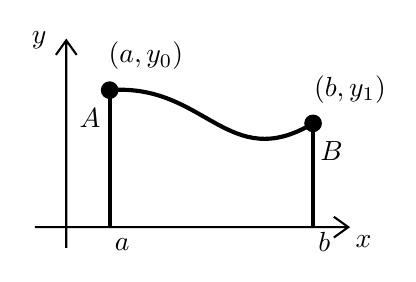
\begin{tikzpicture}[x=0.75pt,y=0.75pt,yscale=-1,xscale=1]
	%uncomment if require: \path (0,142); %set diagram left start at 0, and has height of 142
	
	%Shape: Axis 2D [id:dp8399462359464056] 
	\draw  (57,105) -- (208,105)(72.1,15) -- (72.1,115) (201,100) -- (208,105) -- (201,110) (67.1,22) -- (72.1,15) -- (77.1,22)  ;
	%Straight Lines [id:da20683963263238114] 
	\draw [line width=1.5]    (93,39) -- (93,105.5) ;
	%Straight Lines [id:da0899968561040092] 
	\draw [line width=1.5]    (191,55) -- (191,105.5) ;
	%Shape: Circle [id:dp7209568664487347] 
	\draw  [fill={rgb, 255:red, 0; green, 0; blue, 0 }  ,fill opacity=1 ] (89.25,39) .. controls (89.25,36.93) and (90.93,35.25) .. (93,35.25) .. controls (95.07,35.25) and (96.75,36.93) .. (96.75,39) .. controls (96.75,41.07) and (95.07,42.75) .. (93,42.75) .. controls (90.93,42.75) and (89.25,41.07) .. (89.25,39) -- cycle ;
	%Shape: Circle [id:dp9856565480799604] 
	\draw  [fill={rgb, 255:red, 0; green, 0; blue, 0 }  ,fill opacity=1 ] (187.25,55) .. controls (187.25,52.93) and (188.93,51.25) .. (191,51.25) .. controls (193.07,51.25) and (194.75,52.93) .. (194.75,55) .. controls (194.75,57.07) and (193.07,58.75) .. (191,58.75) .. controls (188.93,58.75) and (187.25,57.07) .. (187.25,55) -- cycle ;
	%Curve Lines [id:da8499791485244599] 
	\draw [line width=1.5]    (93,39) .. controls (139,35.5) and (150,79.5) .. (191,55) ;
	
	% Text Node
	\draw (94,108.9) node [anchor=north west][inner sep=0.75pt]    {$a$};
	% Text Node
	\draw (192,105.9) node [anchor=north west][inner sep=0.75pt]    {$b$};
	% Text Node
	\draw (210,107.4) node [anchor=north west][inner sep=0.75pt]    {$x$};
	% Text Node
	\draw (54,9.4) node [anchor=north west][inner sep=0.75pt]    {$y$};
	% Text Node
	\draw (91,14.4) node [anchor=north west][inner sep=0.75pt]    {$( a,y_{0})$};
	% Text Node
	\draw (190,30.4) node [anchor=north west][inner sep=0.75pt]    {$( b,y_{1})$};
	% Text Node
	\draw (77,46.15) node [anchor=north west][inner sep=0.75pt]    {$A$};
	% Text Node
	\draw (193,62.15) node [anchor=north west][inner sep=0.75pt]    {$B$};
	
	
\end{tikzpicture}

Итак минимизируемый функционал
\begin{equation*}
	\hfill\J[y]=\int\limits_a^b\sqrt{1+y^{\prime2}}\,dx,\quad
	\K\left\{y(x)|y\in\Cfn[{[a,b]}]{1}\ y(a)=y_0,\,y(b)=y_1,\ \int\limits_a^b y\,dx=S\right\}_{\displaystyle.}\hfill
\end{equation*}
Ищем $\min\limits_{y\in\K}\,\J[y]$. Для функционала $\J_1[y]=\smallint\limits_a^b y\,dx$ значение $S$ --- не экстремальное, поэтому применима общая теория
\begin{equation*}
	\hfill F^{\ast}\eqdef\sqrt{1+y^{\prime2}}-\lambda\cdot y\quad\Rightarrow\quad F^{\ast}_{y}-\der{}{x}F^{\ast}_{y'}=0.\hfill
\end{equation*}
Так как $F^{\ast}$ не содержит $x$, то уравнение Эйлера имеет первый интеграл $F^{\ast}-y'\cdot F^{\ast}_{y'}=c_1$, то есть
\begin{gather*}
	\sqrt{1+y^{\prime2}}-\lambda\cdot y-\frac{y^{\prime2}}{\sqrt{1+y^{\prime2}}}=c_1\quad\Rightarrow\quad
	\frac{1}{\sqrt{1+y^{\prime2}}}=c_1+\lambda\cdot y\quad\Rightarrow\quad\frac{1}{(c_1+\lambda\cdot y)^2}=1+y^{\prime2}\quad\Rightarrow\\\Rightarrow\quad y'=\pm\sqrt{\frac{1}{(c_1+\lambda\cdot y)^2}-1}=\pm\frac{\sqrt{1-(c_1+\lambda\cdot y)^2}}{c_1+\lambda\cdot y}\quad\Rightarrow\quad\der{x}{y}=\pm\frac{c_1+\lambda\cdot y}{\sqrt{1-(c_1+\lambda\cdot y)^2}}\quad\Rightarrow\\\Rightarrow\quad x+c_2=\pm\sqrt{1-(c_1+\lambda\cdot y)^2}\bigm/\lambda\quad\Rightarrow\quad (x+c_2)^2+(y+c_3)^2=1\bigm/\lambda^2
\end{gather*}
остальное --- дело техники.
\section[Квадратичный функционал. Оператор Штурма.]{Квадратичный функционал. Оператор Штурма--Лиувилля.}
\label{lecture4section2}
Рассмотрим функционал
\begin{equation*}
	\hfill\J[y]=\int\limits_a^b\Big(Q\cdot y^{\prime2}+P\cdot y^2\Big)\,dx,\hfill
\end{equation*}
\begin{equation*}
	\text{где }Q(x)\in\Cfn[{[a,b]}]{1},\ Q(x)>0,\,x\neq a,\ P(x)\in\Cfn[{[a,b]}]{},\text{ или }P(x)\geqslant0,\ P(x)\in\Cfn[{(a,b]}]{}.
\end{equation*}
\begin{equation*}
	\text{Класс функций }\K=\left\{y(x)|y\in\Cfn[{[a,b]}]{1},\ y(a)=y(b)=0,\ \int\limits_a^b y^2\,dx=1\right\}_{\displaystyle.}
\end{equation*}
Покажем, что $\min\limits_{y\in\K}\,\J[y]>-\infty$, то есть задача отыскания $\min\limits_{y\in\K}\,\J[y]$ имеет смысл. Очевидно
\begin{equation*}
	\J[y]\geqslant\int\limits_a^b P\cdot y^2\,dx\geqslant P_0>-\infty,\text{ где }P_0=\inf\limits_{x\in[a,b]}\,P(x).
\end{equation*}
Далее, значение $\J_1[y]=\smallint\limits_a^b y^2\,dx=1$ --- не является экстремальным для функционала $\J_1[y]$, поэтому применима общая теория решения изопериметрических задач. 
\begin{equation*}
	\text{Положим }F^{\ast}\eqdef F-\lambda\cdot G=Q\cdot y^{\prime2}+P\cdot y^2-\lambda\cdot y^2
\end{equation*}
и напишем для $F^{\ast}$ уравнение Эйлера
\begin{equation*}
	\hfill 2\cdot P\cdot y-2\cdot\lambda\cdot y-2\cdot\der{}{x}\Big(Q\cdot y'\Big)=0\hfill
\end{equation*}
или
\begin{equation}
	\label{l4:eq:22}
	\hfill-\der{}{x}\Big(Q\cdot y'\Big)+P\cdot y=\lambda\cdot y.\hfill
\end{equation}
Решение~\eqref{l4:eq:22} ищем в классе $y(x)\in\Cfn[{[a,b]}]{2}$, $y(a)=y(b)=0$.

\noindent Выражение в левой части~\eqref{l4:eq:22} называется оператором Штурма--Лиувилля $\LL y$, то есть~\eqref{l4:eq:22} запишется в виде 
\begin{equation}
	\label{l4:eq:23}
	\hfill \LL y=\lambda\cdot y.\hfill
\end{equation}
Оператор $\LL$ рассматривается в области 
\begin{equation*}
	\hfill\mc{D}_{\LL}=\left\{y(x)|y\in\Cfn[{[a,b]}]{2},\ y(a)=y(b)=0\right\}_{\displaystyle.}\hfill
\end{equation*}
Очевидно, что оператор \LL{} --- линейный, и решения~\eqref{l4:eq:23} --- это собственные функции, отвечающие собственному значению $\lambda$.

Далее мы займёмся изучением свойств собственных функций и собственных значений в~\eqref{l4:eq:23}. Для того, чтобы понять, что можно ожидать в общем случае, мы рассмотрим сначала случай постоянных коэффициентов: $Q=c_1$, $P=c_2$, причём $Q>0$, а в качестве отрезка $[a,b]$ возьмём отрезок $[0,l]$. Таким образом мы приходим к задаче
\begin{equation}
	\label{l4:eq:24}
	\hfill-c_1\cdot y''+c_2\cdot y=\lambda\cdot y\quad\Rightarrow\quad y''+\frac{\lambda-c_2}{c_1}\cdot y=0,\hfill
\end{equation}
при $y(0)=y(l)=0$.

\noindent Обозначим $\omega^2\eqdef(\lambda-c_2)\bigm/c_1$ и покажем, что $\omega^2>0$\footnote{Мы пока не знаем, может быть $\omega^2$ --- не вещественно.}. 

\noindent Умножим~\eqref{l4:eq:24} на $\overline{y}$ и проинтегрируем по $[0,l]$. 
\begin{gather*}
	\text{Тогда так как }\int\limits_0^l \underbrace{\overline{y}}_{u}\cdot \underbrace{y''\,dx}_{dv}=\underbrace{y'\cdot \overline{y}\mathop{\Big|}\limits_0^l}_{\lefteqn{\substack{\scriptstyle	=0, \text{ ибо }\\
				y(0)=y(l)=0}}}-\int\limits_0^l|y'|^2\,dx=-\int\limits_0^l|y'|^2\,dx\text{ то получим }\\
	-\int\limits_0^l|y'|^2\,dx+\omega^2\cdot\int\limits_0^l|y|^2\,dx=0,\text{ то есть }\omega^2\geqslant0.
\end{gather*}
При $\omega=0$ получаем $y'\equiv0$, то есть $y=const$, но $y(0)=0$. Значит $y\equiv0$, что нас не устраивает, поэтому $\omega^2>0$.

Таким образом~\eqref{l4:eq:24} приобретает вид
\begin{equation*}
	\hfill y''+\omega^2\cdot y=0\hfill
\end{equation*}  
и решение
\begin{equation*}
	\hfill y(x)=d_1\cdot\sin\big(\omega\cdot x\big)+d_2\cdot\cos\big(\omega\cdot x\big).\hfill
\end{equation*}
Так как $y(0)=0$, то $d_2=0$. Так как $y(l)=0$, то $d_1\cdot\sin\big(\omega\cdot l\big)=0$. Поскольку $d_1\neq0$ (иначе $y(x)\equiv0$), то $\sin\big(\omega\cdot l\big)=0$ и значит $\omega\cdot l=\pi\cdot k$, $k=1,\ldots$ 
\begin{equation*}
	\text{Откуда }\omega_k=\frac{\pi\cdot k}{l},\quad \frac{\lambda_k-c_2}{c_1}=\left(\frac{\pi\cdot k}{l}\right)^2,\quad\lambda_k=c_1\cdot\left(\frac{\pi\cdot k}{l}\right)^2+c_2,
\end{equation*}
а собственные функции $y_k=d_{1k}\cdot\sin\left(\frac{\pi\cdot k}{l}\cdot x\right)$. Для выполнения изопериметрического условия считаем
\begin{equation*}
	\int\limits_0^l y_k^2\,dx=d_{1k}^2\cdot\int\limits_0^l\left(\sin\left(\frac{\pi\cdot k}{l}\cdot x\right)\right)^2\,dx=d_{1k}^2\cdot\int\limits_0^l\frac{1-\cos\left(\frac{2\cdot\pi\cdot k}{l}\cdot x\right)}{2}\,dx=d_{1k}^2\cdot\frac{l}{2}=1,
\end{equation*}
откуда $d_{1k}=\pm\displaystyle\sqrt{\frac{2}{l}}$. Окончательно получаем, что
\begin{equation*}
	\hfill y_k=\pm\sqrt{\frac{2}{l}}\cdot\sin\left(\frac{\pi\cdot k}{l}\cdot x\right),\quad\lambda_k=c_1\cdot\left(\frac{\pi\cdot k}{l}\right)^2+c_2.\hfill
\end{equation*}
Что мы узнали в нашем частном случае:
\begin{enumerateD}
	\item\label{l4:enum:1} Собственные значения --- вещественны.
	\item Собственные значения $\lambda_k$ стремятся к $\infty$ со скоростью $k^2$.
	\item Собственные пространства $\displaystyle \Ul[\lambda_k]$, отвечающие собственным значениям $\lambda_k$ --- одномерны (или по-другому: каждому собственному значению отвечает единственная --- с точностью до знака--- собственная функция, для которой выполнено изопериметрическое условие).
	\item Собственные функции $y_k$ и $y_m$, отвечающие различным собственным значениям $\lambda_k\neq\lambda_m$ удовлетворяют соотношению
	\begin{equation*}
		\hfill\int\limits_0^l y_k\cdot y_m\,dx=0,\quad k\neq m.\hfill
	\end{equation*}
	\item\label{l4:enum:5} Из теории рядов Фурье следует, что если $y(x)\in\Cfn[{[0,l]}]{2}$ и $y(0)=y(l)=0$, то 
	\begin{equation*}
		\hfill y(x)=\sum\limits_{k=1}^{\infty} A_k\cdot\sin\left(\frac{\pi\cdot k}{l}\cdot x\right),\hfill
	\end{equation*}
	где $A_k$ --- коэффициенты Фурье и ряд по собственным функциям сходится равномерно. 
\end{enumerateD}

Мы выяснили, что можно ожидать от свойств собственных значений и собственных функций оператора Штурма. Далее мы установим, что и в случае переменных (а не постоянных!) коэффициентов $Q(x)$ и $P(x)$ выполняются утверждения~\ref{l4:enum:1}--\ref{l4:enum:5}